\documentclass[11pt, oneside]{article}   	% use "amsart" instead of "article" for AMSLaTeX format
\usepackage{geometry}                		% See geometry.pdf to learn the layout options. There are lots.
\geometry{letterpaper}                   		% ... or a4paper or a5paper or ... 
%\geometry{landscape}                		% Activate for rotated page geometry
%\usepackage[parfill]{parskip}    		% Activate to begin paragraphs with an empty line rather than an indent
\usepackage{graphicx}				% Use pdf, png, jpg, or eps§ with pdflatex; use eps in DVI mode
								% TeX will automatically convert eps --> pdf in pdflatex		
\usepackage{amssymb}

%SetFonts

%SetFonts
\setlength{\parindent}{0pt}

\title{Summary of Neural Networks to Predict the Market Paper and Tutorial by Vivek Palaniappan}
\author{Jody Shu}
%\date{}							% Activate to display a given date or no date

\begin{document}
\begin{Large}
\maketitle
%\section{}
%\subsection{}

This article will be an introduction on how to use neural networks to predict the stock market, in particular the price of a stock (or index).  \\

The author follows the step from data acquisition, data preprocessing (split up into train and test set, and each window size has sample size 10).  After that, the author use multiplayer perceptron (MLP) and the Long Short Term Model (LSTM).  The different between MLP and LSTM is that MLP has no ability to analyze the relationship between batch of data and LSTM has the ability to store certain information about the data for later use.  LSTM is a special kind of Recurrent Neural Networks (RNNs).  In a general RNNs, there is a problem which is that it suffers from the vanishing gradient problem because as the layers increase, the gradient decrease.  However, this problem is solved by using LSTMs.

The author implement the LSTMs/MLP by using keras Python package which adding layers to the network instead of defining the entire network at once.  The author normalizes the data by divide it by 200, so the weights in the neural network do not grow too large.  The Adam optimizer is chosen because it takes advantages of Root Mean Square Propagation and Adaptive Gradient Algorithm.  After that, the author feed the training data into the model, and use test data to evaluate how well the model perform after it is trained.  Once the author evaluate the test data, he used a new set of data and run the algorithm and 'backtesting the Model', and the prediction stock price is pretty good as you can see the graph below.  

\begin{figure}[h] %  figure placement: here, top, bottom, or page
   \centering
   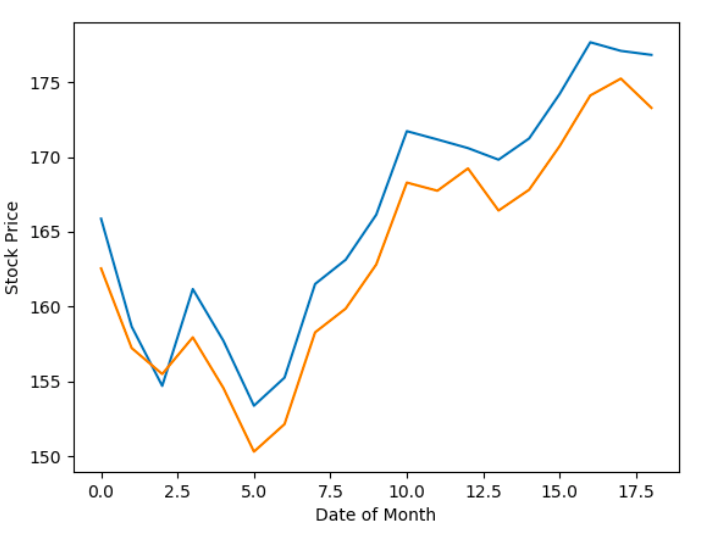
\includegraphics[width=6in]{prediction_plot} 
\end{figure}


\end{Large}
\end{document}


